% chktex-file 44 32 36 38 18 11 8 26

\pagestyle{DS_FP}
%\NomPrenomNote{}


\medskip

\emph{Dans ce sujet, vous arrondirez toutes les valeurs à $10^{-4}$ si nécessaire.}


\section*{PARTIE A~--~Etude d'une batterie de secours (Fonctions)}

Lors d'une coupure de courant, la capacité restante $f(t)$ (en Wh) d'une batterie de secours en fonction du temps $t$ (en heures) est modélisée par:

\fbox{$f(t)=(at+b)\e^{-t}$} \quad $f(t)$ représente la capacité restante en Wh après $t$ heures. $a$ et $b$ sont des constantes réelles.

On constate que:
\begin{itemize}
    \item Au début de la coupure de courant, la capacité de la batterie de secours est de \fbox{120 Wh}.
    \item La tangente à la courbe représentative de $f$ au point d'abscisse 0 coupe l'axe des abscisses au point \fbox{(1.2; 0)}.
\end{itemize}

 \begin{enumerate}[resume=monDS]

        
     \item En utilisant les informations données dans l'énoncé, déterminer à l'aide de Géogébra les valeurs de $a$ et $b$. \hfill\reponseLigne[5cm]{\texttt{$a=20$ et $b=120$}} 

    \appelprof{}
\end{enumerate}

\bigskip

Dans la suite de l'exercice, on considère que \fbox{$f(t)=20(t+6)\e^{-t}$} et que la fonction dérivée de $f$ est de la forme \fbox{$f'(t)=-20(t+5)\e^{-t}$}.

\begin{enumerate}[resume=monDS]

        \item Etudier les variations de $f$ sur $\ff{0}{+\infty}$.
        \begin{blocvisiblex}[height=5]
        {\quad}
        $f'(t)$ est strictement négative sur $\ff{0}{+\infty}$, ainsi $f$ est strictement décroissante sur $\ff{0}{+\infty}$.

         \end{blocvisiblex}

         \medskip
         \item On considère que la situation est critique lorsque la capacité de la batterie de secours est inférieure à \fbox{20 Wh}. Déterminer à l'aide de Géogébra à partir de combien d'heures (arrondi à $10^{-4}$) la situation devient critique.
            \begin{blocvisiblex}[height=1.2]
            {\quad}
            La situation est critique sur à partir de $2,0907$ heures.
             \end{blocvisiblex}
\end{enumerate}

             \medskip
             On suppose qu'une primitive de $f$ est donnée par \fbox{$F(t)=-20(t+7)\e^{-t}$}
\begin{enumerate}[resume=monDS]

             \medskip

                 \item Quelle formule permettrait de calculer la capacité moyenne de la batterie de secours sur l'intervalle $\ff{0}{5}$?
                    \begin{blocvisiblex}[height=1.5]
    {
    \faSquare[regular] \, $\dfrac{1}{5}\big(F(0) - F(5)\big)$ \hfill \faSquare[regular] \, $\dfrac{1}{5}\big(F(5) - F(0)\big)$ \hfill \faSquare[regular] \, $\dfrac{1}{5}\big(F(5)\big)$ \hfill \faSquare[regular] \, $\dfrac{1}{5}\big(F(0)\big)$ \hspace{1cm} 
 }         
    \faSquare[regular] \, $\dfrac{1}{5}\big(F(0) - F(5)\big)$ \hfill \faCheck[regular] \, $\dfrac{1}{5}\big(F(5) - F(0)\big)$ \hfill \faSquare[regular] \, $\dfrac{1}{5}\big(f(5)-f(0)\big)$ \hfill \faSquare[regular] \, $\dfrac{1}{5}\big(f(0)-f(5)\big)$ \hspace{1cm} 
    \end{blocvisiblex}

                 \medskip
                 \item Calculer alors la capacité moyenne de la batterie de secours sur $\ff{0}{5}$ arrondi à $10^{-2}$ près.
                    \begin{blocvisiblex}[height=1.5]
                    {\quad}
                    La capacité moyenne de la batterie de secours sur $\ff{0}{5}$ est de $\dfrac{1}{5-0}\int_0^5 f(x) \, \dx\approx $ Wh.
                     \end{blocvisiblex}
            
    \end{enumerate}


\medskip

    \section*{PARTIE B~--~Approximation numérique et suites}


    On désire approximer la capacité de la batterie de secours à l'aide d'une suite numérique.

    On note $u_n$ l'énergie restante (en Wh) après $n$ minutes. On suppose que \fbox{$u_0=120$ Wh} et que chaque minute, la batterie perd \fbox{$1,7\%$} de l'énergie qu'il lui reste.


\begin{enumerate}[series=monDS, resume]
    \item Justifier que la suite $(u_n)$ vérifie la relation de récurrence \fbox{$u_{n+1}=0,983\cdot u_n$}.
    \begin{blocvisiblex}[height=3.]
    {\quad}
    La suite $(u_n)$ vérifie la relation de récurrence $u_{n+1}=0,983\cdot u_n$ car à chaque minute, la batterie perd $1,7\%$ de l'énergie qu'elle lui reste.

    On a donc $u_{n+1}=u_n-0,017\cdot u_n=0,983\cdot u_n$.

    \end{blocvisiblex}
    \medskip
    \item Déterminer la nature de la suite $(u_n)$. Donner son premier terme et sa raison. 
    \begin{blocvisiblex}[height=2]
    {\quad}

    La suite $(u_n)$ est de la forme $u_{n+1}=q \times u_n$ avec $q=0,983$ constant, donc c'est une suite géométrique de raison $0,983$ et de premier terme $u_0=120$.
    \end{blocvisiblex}
    \medskip
    \item Exprimer $u_n$ en fonction de $n$. 
    \begin{blocvisiblex}[height=1.5]
    {\quad}
    $(u_n)$ est une SG de raison $0,983$ et de premier terme $u_0=120$, donc pour tout $n$ entier naturel, on a $u_n=u_0 \times q^n=120 \times 0,983^n$.
    \end{blocvisiblex}
    \medskip

    \begin{minipage}{0.44\textwidth}
            \item Compléter le script suivant qui détermine après combien de minutes l'énergie sera inférieure à \fbox{100 Wh}.

    \end{minipage}\hfill{}
    \begin{minipage}{0.48\textwidth}
\begin{tcblisting}{%
  listing only,
  colback=white, 
  colupper=black, 
  title=Algorithme de recherche de seuil,
  boxsep=0pt,
  left=5mm,
  listing options={
    numbers=none,
    basicstyle=\ttfamily,
    escapeinside={(*}{*)},
    literate={<-}{{$\bm{\leftarrow}$}}2, % Ajout d'un petit espace après la flèche
    frame=none % Supprime le cadre interne de listings
    }
}
n <- 0
u <- 120
tant que (*\trou{u >= 100}*):
        u <- (*\trou{0,983 * u}*)
        n <- (*\trou{n + 1}*)
afficher (n)
\end{tcblisting}
    \end{minipage}

    

\medskip

\item A l'aide de Géogébra, déterminer après combien de minutes l'énergie sera inférieure à \fbox{100 Wh}.
\begin{blocvisiblex}[height=1]
{\quad}
On trouve $n=10$ donc après 10 minutes, l'énergie sera inférieure à 100 Wh.
\end{blocvisiblex}

\appelprof{}
\end{enumerate}

\pagebreak

\section*{PARTIE C~--~Analyse de trafic et erreurs de trames}


\medskip

 \begin{minipage}{0.65\textwidth}
On constate que\begin{itemize}
    \item $80\%$ des trames proviennent du Réseau 1.
    \item $20\%$ des trames proviennent du Réseau 2.
    \item La probabilité qu'une trame du réseau 1 soit corrompue est de $0,02$.
    \item La probabilité qu'une trame du réseau 2 soit corrompue est de $0,05$.
\end{itemize}

On considère une trame au hasard reçue par le serveur et on note:
\begin{itemize}
    \item $C$ l'événement « la trame est corrompue ».
    \item $R_1$ l'événement « la trame provient du Réseau 1 ».
    \item $R_2$ l'événement « la trame provient du Réseau 2 ».
\end{itemize}


\medskip

\begin{enumerate}[series=monDS, resume]
    \item Compléter l'arbre de probabilité ci-contre.
\end{enumerate}

\end{minipage}\hfill{}
\begin{minipage}{0.38\textwidth}
    \begin{blocvisiblex}[height=5]
    {\begin{center}
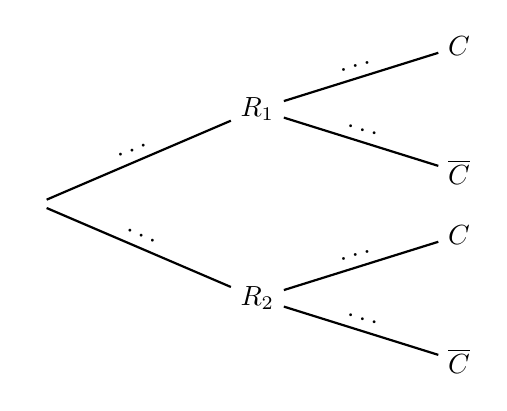
\begin{tikzpicture}[
        scale=0.8,
    grow=right,     % On définit la croissance vers la droite
    % Réglages des distances entre les niveaux et les branches
    level 1/.style={sibling distance=3cm, level distance=3.5cm},
    level 2/.style={sibling distance=2cm, level distance=3.2cm},
    every node/.style={sloped}, % Aligne le texte sur les branches
    edge from parent/.style={draw, thick} % Ajoute une flèche au bout
]
% Racine
\node {} 
    child { node {$R_2$}
        child { node {$\overline{C}$} 
            edge from parent node[above] {$\ldots{}$} }
        child { node {$C$} 
            edge from parent node[above] {$\ldots{}$} }
        edge from parent node[above] {$\ldots{}$} }
    child { node {$R_1$}
        child { node {$\overline{C}$} 
            edge from parent node[above] {$\ldots{}$} }
        child { node {$C$} 
            edge from parent node[above] {$\ldots{}$} }
        edge from parent node[above] {$\ldots{}$} }
    ;
\end{tikzpicture}
\end{center}}
\begin{center}
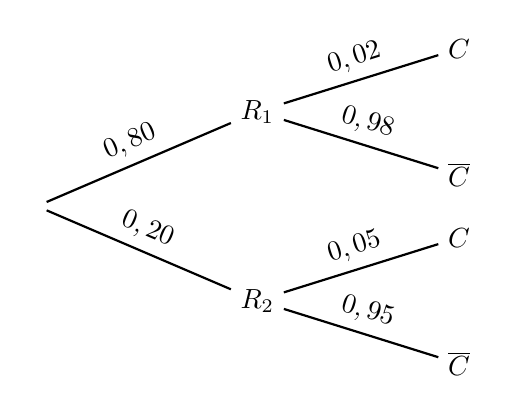
\begin{tikzpicture}[
    scale=0.8,
    grow=right,     % On définit la croissance vers la droite
    % Réglages des distances entre les niveaux et les branches
    level 1/.style={sibling distance=3cm, level distance=3.5cm},
    level 2/.style={sibling distance=2cm, level distance=3.2cm},
    every node/.style={sloped}, % Aligne le texte sur les branches
    edge from parent/.style={draw, thick} % Ajoute une flèche au bout
    %edge from parent/.style={draw, -latex, thick} % Ajoute une flèche au bout
]
% Racine
\node {} 
    child { node {$R_2$}
        child { node {$\overline{C}$} 
            edge from parent node[above] {$0,95$} }
        child { node {$C$} 
            edge from parent node[above] {$0,05$} }
        edge from parent node[above] {$0,20$} }
    child { node {$R_1$}
        child { node {$\overline{C}$} 
            edge from parent node[above] {$0,98$} }
        child { node {$C$} 
            edge from parent node[above] {$0,02$} }
        edge from parent node[above] {$0,80$} }
    ;
\end{tikzpicture}
\end{center}
    \end{blocvisiblex}
\end{minipage}



    
\begin{enumerate}[resume=monDS]
    \item Calculer la probabilité que la trame soit corrompue et provienne du Réseau 2.
     \begin{blocvisiblex}[height=1.5]
    {\quad}
    $P(R_2 \cap C) = P(R_2) \times P_{R_2}(C) = 0,20 \times 0,05 = 0,01$

    \smallskip
    La probabilité que la trame soit corrompue et provienne du Réseau 2 est de $0,01$.
     \end{blocvisiblex}
     \medskip
    \item Calculer $P(C)$ et donner une interprétation à cette valeur dans le contexte de l'énoncé.
    \begin{blocvisiblex}[height=2.5]
    {\quad}
    $P(C)=P(R_1 \cap C)+P(R_2 \cap C)=P(R_1) \times P_{R_1}(C)+P(R_2) \times P_{R_2}(C)=0,80 \times 0,02+0,20 \times 0,05=0,026$

        \smallskip
    La probabilité que la trame soit corrompue est de $0,026$.
    \end{blocvisiblex}
    \medskip
    \item Sachant que la trame est corrompue, calculer la probabilité qu'elle provienne du Réseau 2.
    \begin{blocvisiblex}[height=2]
    {\quad}
    $P_{C}(R_2)=\dfrac{P(R_2 \cap C)}{P(C)}=\dfrac{0,01}{0,026}\approx 0,3846$
        \smallskip
    La probabilité que la trame provienne du Réseau 2 sachant qu'elle est corrompue est d'environ $0,385$.
     \end{blocvisiblex}
    \end{enumerate}
      Le serveur reçoit un paquet de 50 trames. On considère que les trames sont indépendantes et que la probabilité qu'une trame soit corrompue est de $0,026$. On note $X$ le nombre de trames corrompues parmi les 50 trames reçues. On suppose que $X$ suit une loi binomiale de paramètres $n=50$ et $p=0,026$.
     
    \begin{enumerate}[resume=monDS]
        \item Déterminer la probabilité d'avoir au moins 3 trames corrompues dans ce lot.
    \begin{blocvisiblex}[height=1]
    {\quad}
    $P(X\geq 3)\approx 0,1407$.    La probabilité d'avoir au moins 3 trames corrompues dans ce lot est  $0,1407$.
    \end{blocvisiblex}
   

\thispagestyle{DS_LP}
    \item Par le calcul, déterminer la probabilité qu'aucune trame ne soit corrompue dans ce lot.
    \begin{blocvisiblex}[height=1.5]
    {\quad}
    $P(X=0)=\binom{50}{0} \times 0,026^0 \times (1-0,026)^{50} = 0,974^{50} \approx 0,2679$

        \smallskip  
    La probabilité d'avoir exactement 0 trames corrompues dans ce lot est d'environ $0,2679$.
    \end{blocvisiblex}
    \medskip
    \item De manière générale, exprimer en fonction de $n$ la probabilité d'avoir au moins une trame corrompue dans un lot de $n$ trames. En déduire le nombre minimum de trames à prélever pour que la probabilité d'en avoir au moins une soit supérieure à 20\%.
    \begin{blocvisiblex}[height=2]
    {\quad}
    $P(X\geq 1)=1-P(X=0)=1-\binom{n}{0} \times 0,026^0 \times (1-0,026)^n = 1-(1-0,026)^n=1-0,974^n$  

    Il faut prélever au moins 8 trames pour que la probabilité d'en avoir au moins 1 corrompue soit supérieure à 20\%.
    \end{blocvisiblex}
     \end{enumerate}